\chapter{Example Applications}

This chapter presents several applications of GEX. Those examples are the result of testing during the firmware development, and do not cover the full range of features, but should give the reader some idea about the possibilities.

\section{Frequency Response Measurement}

The frequency response of a filter may be measured with a combination of the ADC and DAC units. The DAC is configured to generate a sine wave as a stimulus for the filter, while the ADC captures the output waveform. By varying the generated frequency and measuring the amplitude, we obtain a frequency response of the filter. If we measured both the input and output, we could calculate the phase shift and produce a real Bode diagram.

\cref{fig:demofilter} depicts a simple test setup with a passive RC filter; its characteristics in the low-pass and high-pass configuration, as obtained with GEX, are shown in \cref{fig:demofilter_cap}.

\begin{figure}[h]
	\centering
	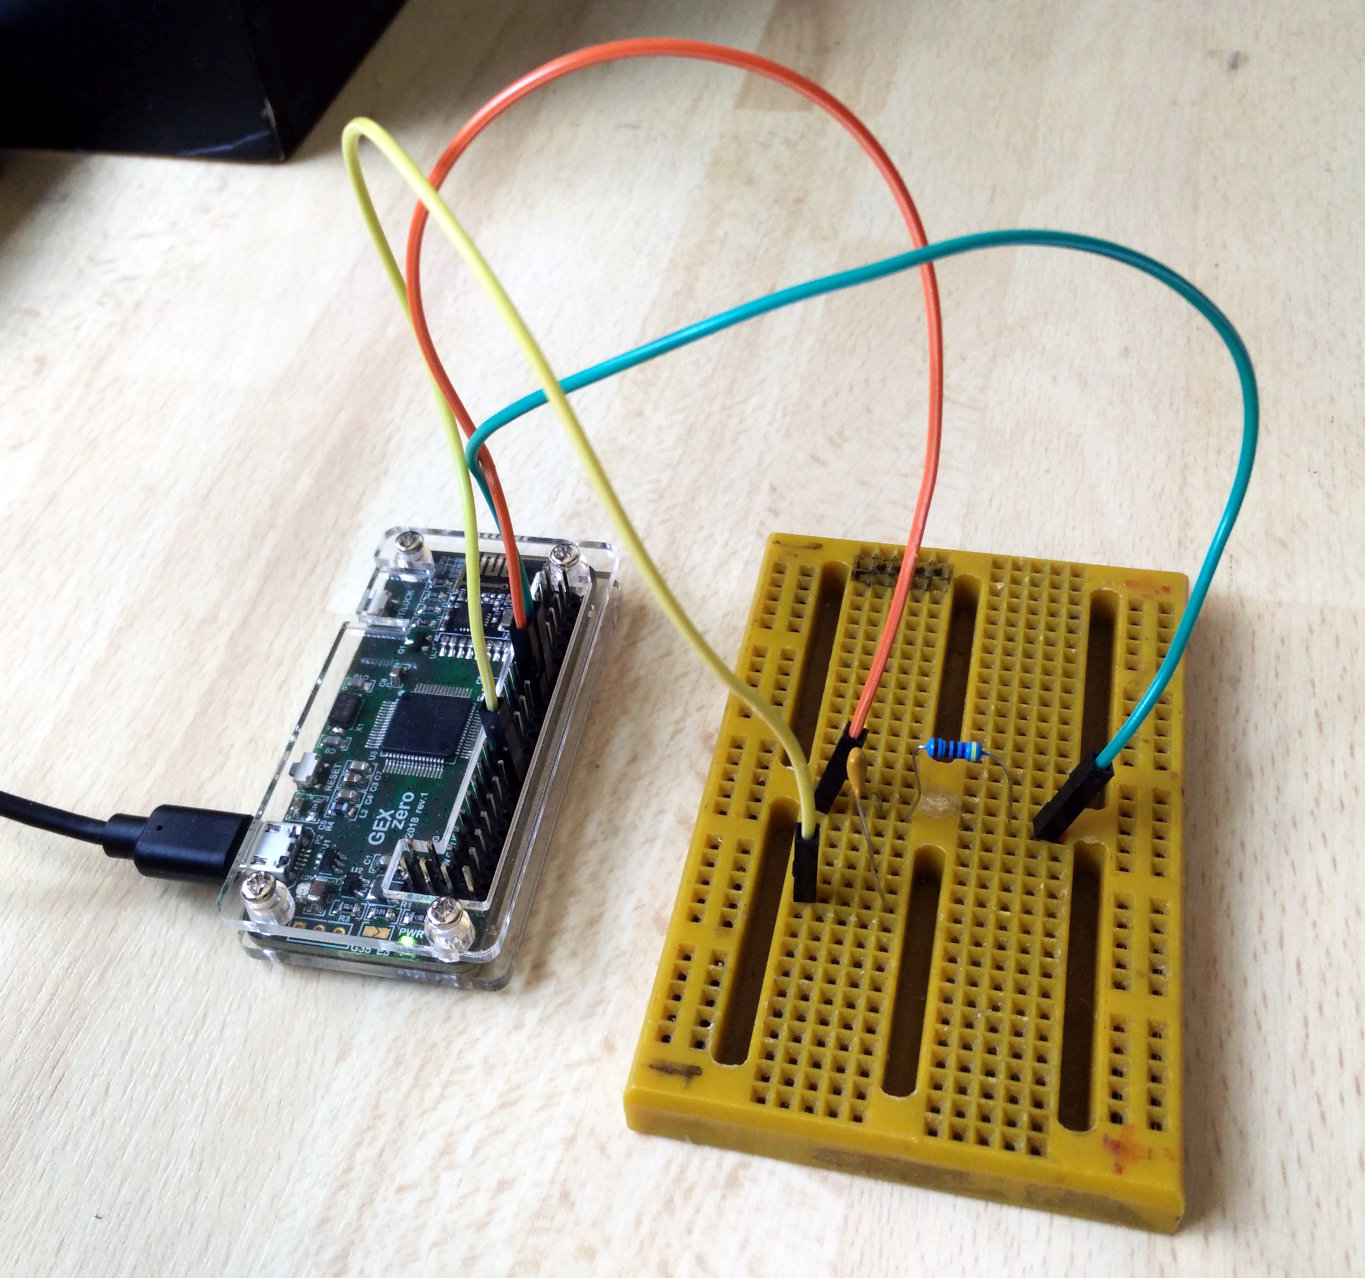
\includegraphics[width=0.6\textwidth]{img/demofilter.jpg}
	\caption{GEX Zero measuring a passive high-pass RC filter}
	\label{fig:demofilter}
\end{figure}

\begin{figure}
	\centering
	\begin{subfigure}{.5\textwidth}
		\centering
		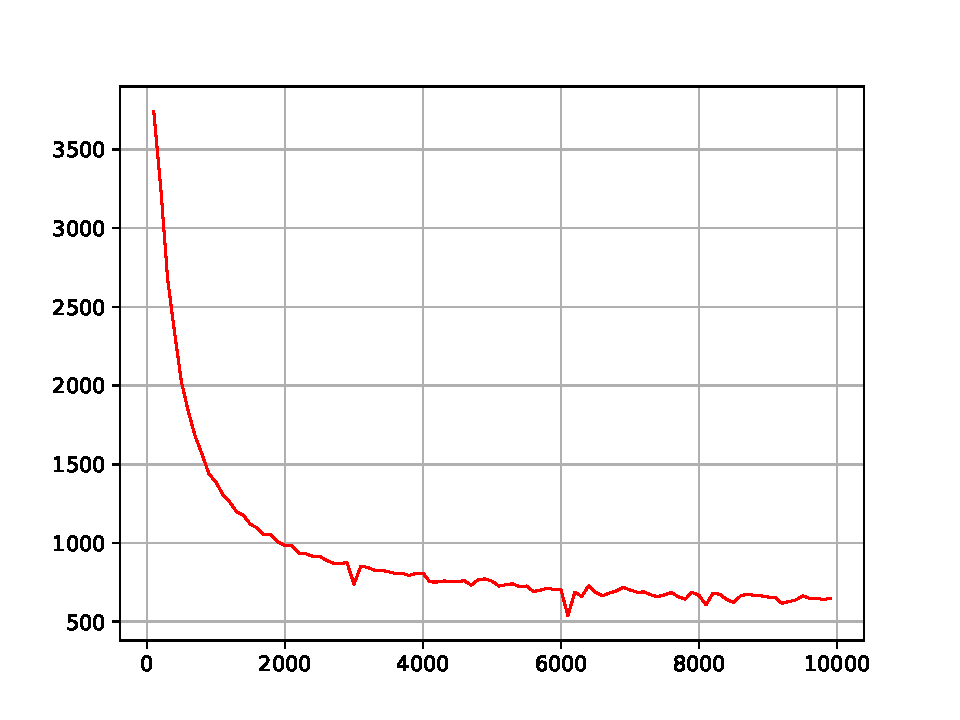
\includegraphics[width=\linewidth]{img/filter1.pdf}
	\end{subfigure}%
	\begin{subfigure}{.5\textwidth}
		\centering
		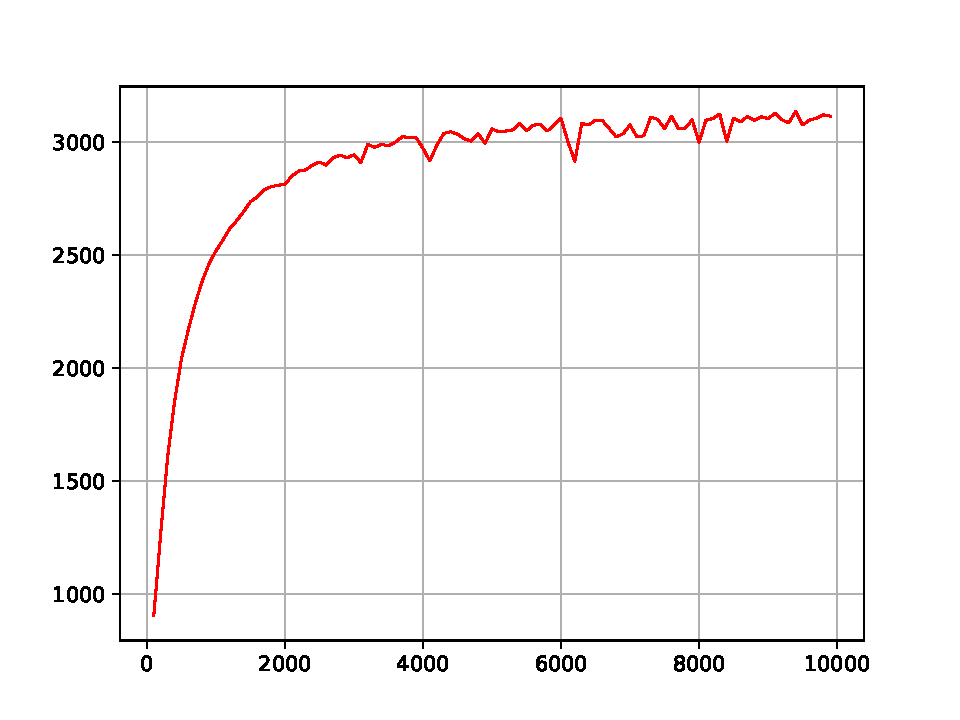
\includegraphics[width=\linewidth]{img/filter2.pdf}
	\end{subfigure}
	\caption[RC filter frequency responses]{Frequency response of two complementary passive RC filters, captured by GEX controlled with a Python script. X: frequency (Hz), Y: peak-to-peak voltage as a raw ADC word }
	\label{fig:demofilter_cap}
\end{figure}

\section{Measuring \texorpdfstring{CO$_2$}{CO2} Concentration}

The \gls{NDIR} CO$_2$ sensor MH-Z19B provides both a \gls{UART} interface, and a pulse-width modulated signal with a duty cycle proportional to the CO$_2$ concentration. 
We used it to verify the duty cycle measurement functionality of the frequency capture unit, and also tested the \gls{USART} unit with the digital interface. The measured concentration was displayed using the SIPO unit on a 74HC595-drive red-green LED bargraph (\cref{fig:democo2}).

\begin{figure}[H]
	\centering
	\begin{subfigure}{.72\textwidth}
		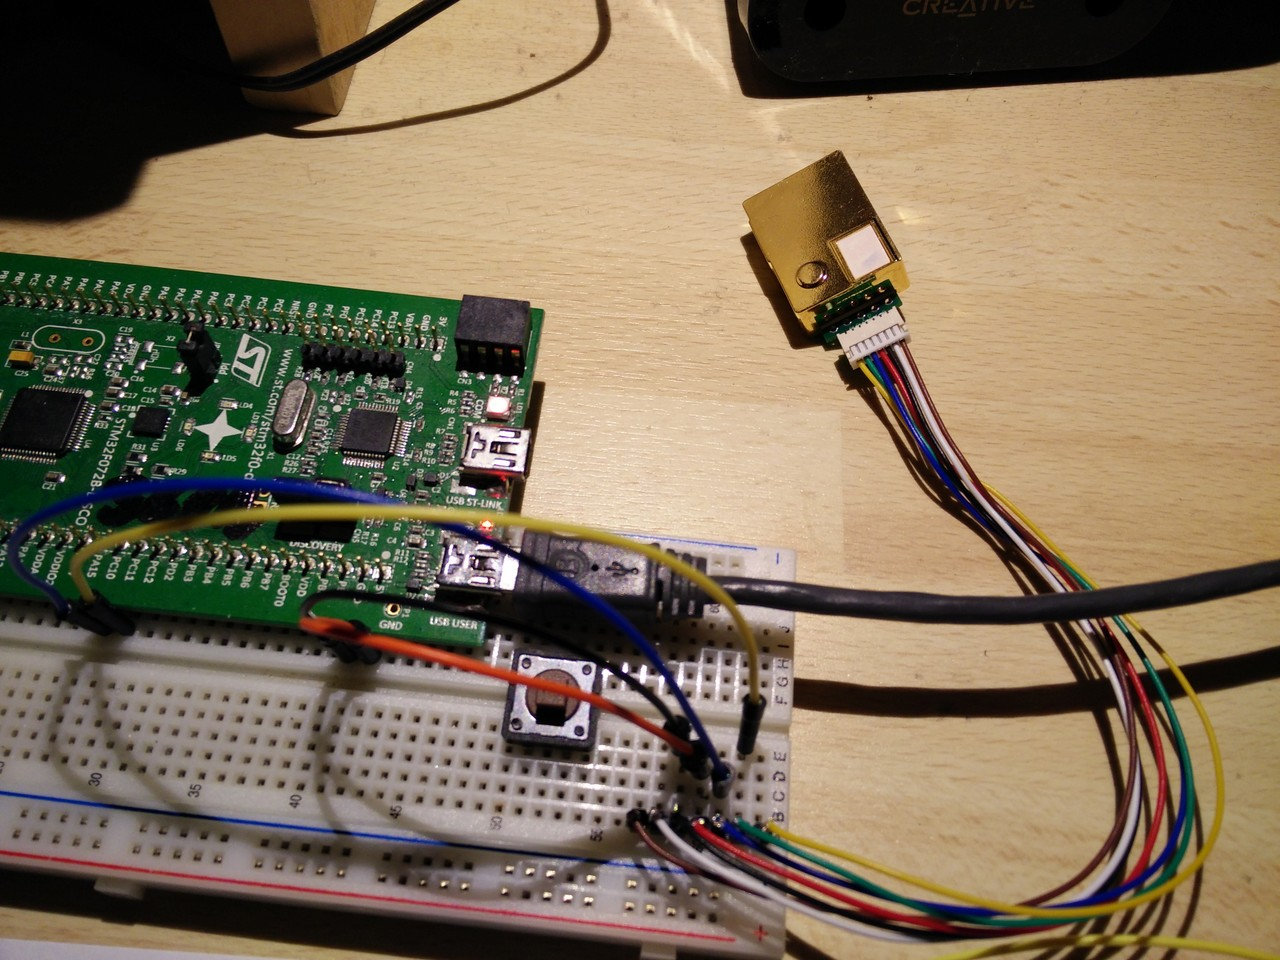
\includegraphics[width=.98\textwidth]{img/ph-co2.jpg}
		\caption{CO$_2$ concentration measurement}
	\end{subfigure}%
	\begin{subfigure}{.28\textwidth}
		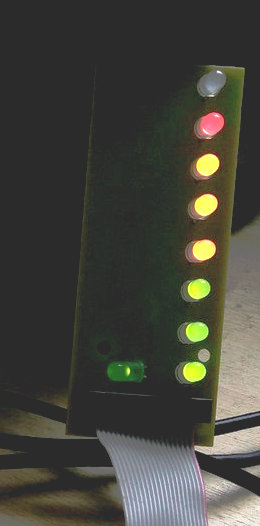
\includegraphics[width=.98\textwidth]{img/sipodemo.jpg}
		\caption{LED display}
	\end{subfigure}
	\caption[Demo with a CO$_2$ sensor]{GEX firmware on the Discovery board reading CO$_2$ concentration from the MH-Z19B \gls{NDIR} sensor and displaying the concentration on an \gls{LED} bargraph}
	\label{fig:democo2}
\end{figure}


\section{Controlling the ``Micro Dot pHAT''}

The ``Micro Dot pHAT'' add-on board was used to test GEX Zero's compatibility with pHATs. A photo of the pHAT on GEX Zero, together with example scripts, was presented in \cref{sec:ex_python_script}. While this board does not provide any useful functionality beyond displaying \gls{LED} patterns, it is a proof that third-party add-ons for the RPi Zero may be compatible with GEX, which introduces many interesting possibilities.

\section{Capturing Transient Effects}

The ADC unit supports level-based triggering. This was tested first by capturing the charging waveform of a capacitor (\cref{fig:captransient}). As the triggering voltage had to be placed above the noise floor, the triggering condition occurred when a part of the waveform already passed. This was solved by using the pre-trigger feature to include past records at the beginning of the capture.

A more interesting application of level triggering was discovered by accident during a thunderstorm, when the electromagnetic interference from a (remote) lightning strike caused a voltage spike to appear on an oscilloscope probe. Investigating the phenomenon, we devised a simple ``lightning trap'' circuit (\cref{fig:lightningtrap}). The resistor forms a discharge path for the capacitor, which acts as a high-pass filter of sorts. The voltage on the \gls{ADC} input remains at about half of the operating range, and lightning strikes produce bursts of voltage spikes which we can trigger on and record.

This method of lightning detection should be regarded as a mere curiosity without much scientific value, and the circuit could certainly be improved to be safer and more sensitive. Nonetheless, the simple setup proved functional and several lightning strikes were automatically captured (\cref{fig:strikes}). 

\begin{figure}[h]
\centering
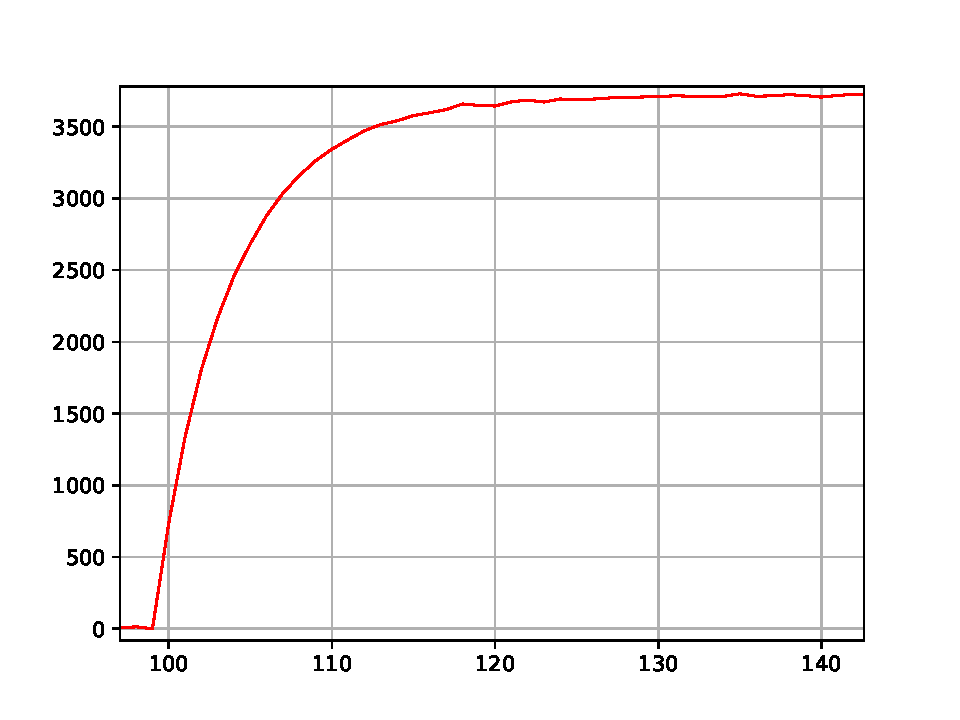
\includegraphics[width=\textwidth]{img/transient.pdf}
\caption{Capacitor charging waveform captured by the ADC unit, 50\,kS/s. X: sample number, Y: ADC word. X grid: 200\,$\mu$s.}
\label{fig:captransient}
\end{figure}

\begin{figure}[b]
\centering
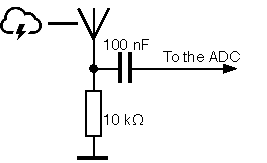
\includegraphics[scale=1.2]{img/thundertrap.pdf}
\caption{The ``lightning trap'' circuit}
\label{fig:lightningtrap}
\end{figure}

\begin{figure}[h]
	\centering
	\begin{subfigure}{.5\textwidth}
		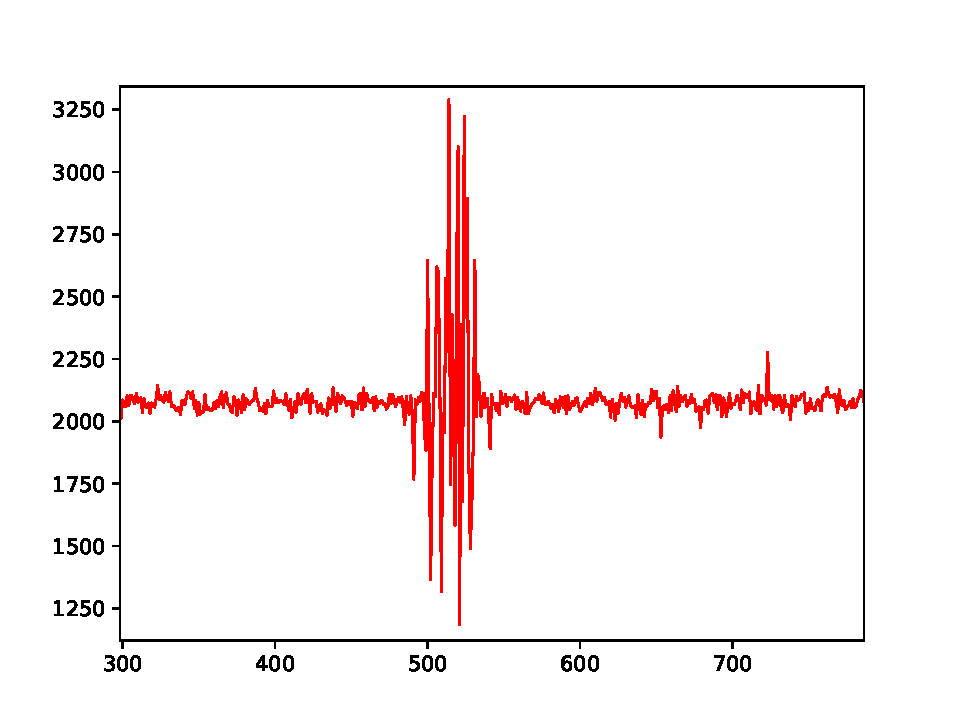
\includegraphics[width=\textwidth]{img/strike1}
	\end{subfigure}%
	\begin{subfigure}{.5\textwidth}
		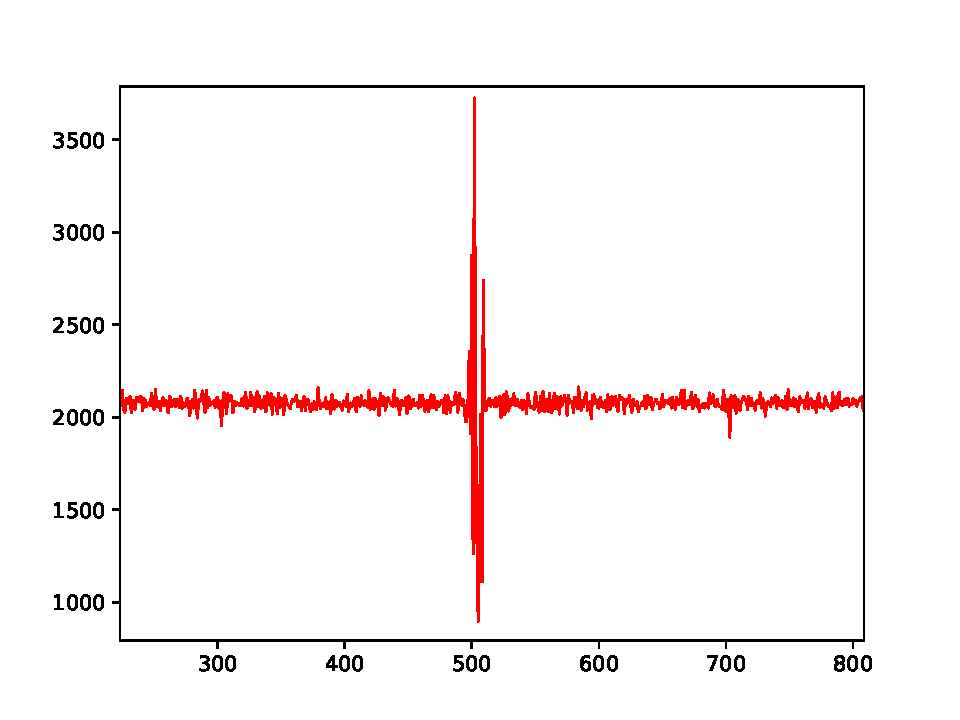
\includegraphics[width=\textwidth]{img/strike2}
	\end{subfigure}\\
	\begin{subfigure}{.5\textwidth}
	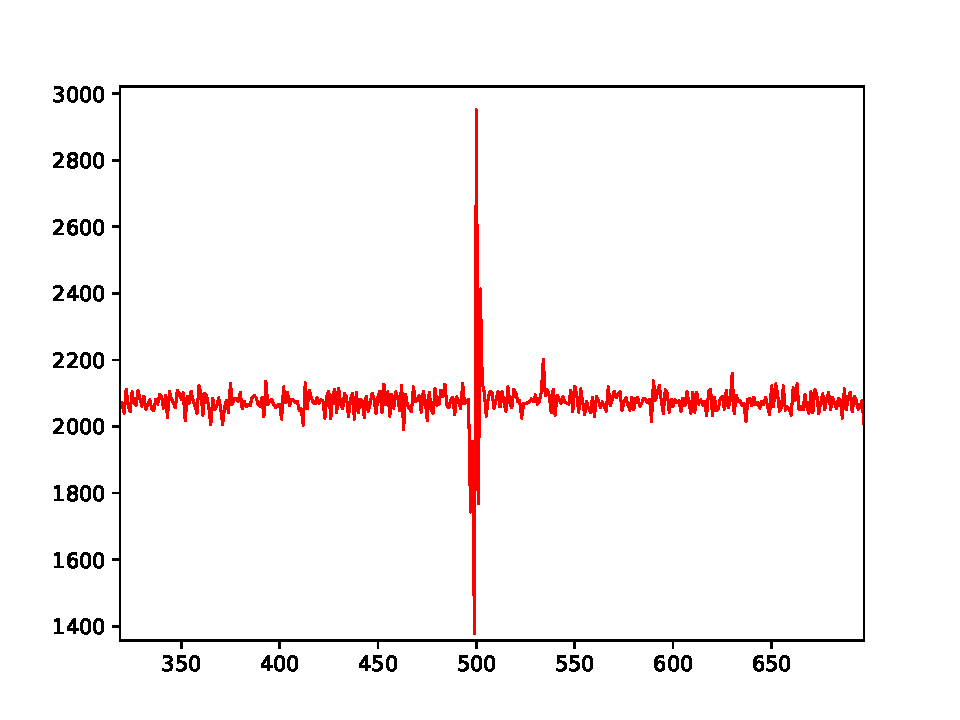
\includegraphics[width=\textwidth]{img/strike3}
	\end{subfigure}%
	\begin{subfigure}{.5\textwidth}
	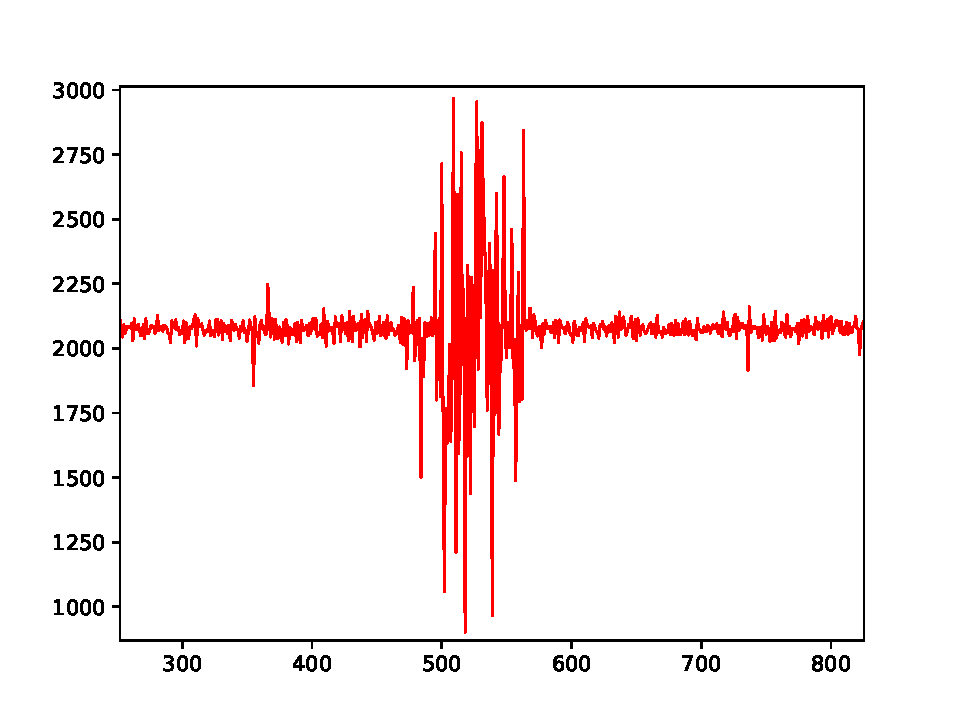
\includegraphics[width=\textwidth]{img/strike4}
	\end{subfigure}
	\caption{Lightning strike-generated bursts of energy captured by the ADC unit. Note the X-axis value 500 where the bursts start: that was the configured pre-trigger length}
	\label{fig:strikes}
\end{figure}










